\documentclass[border=7pt]{standalone}
\usepackage{tikz}
\begin{document}
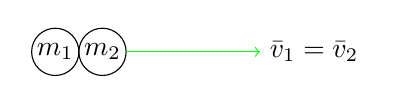
\begin{tikzpicture}
  \draw (4.4,-4) circle [radius=0.3]  node {$m_1$};
  \draw (5,-4) circle [radius=0.3]  node {$m_2$};
  \draw [green, ->] (5.3,-4) -- (7,-4) node [black, right] {$\bar{v}_1 =\bar{v}_2 $};
\end{tikzpicture}
\end{document}
